%!TEX program = xelatex
\documentclass[11pt, a4paper, oneside, UTF8]{ctexbook}
\usepackage{amsmath, amsthm, amssymb, bm, graphicx, hyperref, mathrsfs}
\usepackage[dvipsnames]{xcolor}
\usepackage{tikz}
\usetikzlibrary{backgrounds,arrows,shapes,tikzmark,calc}
\usepackage{geometry}
\usepackage{annotate-equations}
\usepackage{extarrows}
\usepackage{thmbox}

\usepackage{graphicx}
% Custom environments and commands
\newenvironment{note}
{\par\textcolor{blue}{\bfseries Note:}\itshape}{\par}
\newenvironment{remark}
{\par\textcolor{blue}{\bfseries Remark:}\itshape}{\par}
\newtheorem[M]{theorem}{Theorem}[section]
\newtheorem[M]{lemma}[theorem]{Lemma}
\newtheorem[M]{definition}{Definition}[section]
\newtheorem[M]{property}{Property}[section]
\renewcommand{\eqnannotationfont}{\bfseries\small}

\title{{\Huge{\textbf{GACD}}}\\------Teacher Wu}
\author{ManJack}
\date{\today}
\linespread{1.5}

\geometry{
  a4paper,
  total={170mm,257mm},
  left=20mm,
  top=20mm,
}

\begin{document}

\maketitle

\pagenumbering{roman}
\setcounter{page}{1}

\newpage
\begin{center}
	\Huge\textbf{前言}
\end{center}

This is a GACD note-book for xupt. If there has much error in note-book,forgive me. It's just writes for me.

\begin{flushright}
	\begin{tabular}{c}
		ManJack \\
		\today
	\end{tabular}
\end{flushright}

\newpage
\tableofcontents
\newpage
\pagenumbering{arabic}
\setcounter{page}{1}


% Start your content here

\chapter{Linear Equations}
\section{环和域}
\subsection{加群和环的定义}
\begin{definition}[\textbf{加群}]
	假如一个\textbf{Abel群}的代数运算为加法,并且用符号‘+’表示,则该群叫做\textbf{加群}。

\end{definition}

\begin{remark}
	加群的单位元e是唯一的,且e=0。称作\textbf{零元},我们有以下的计算规则:
	\[
		0+a=a+0=a
	\]
\end{remark}

\begin{definition}[\textbf{环}]
	一个集合R称之为环满足:
	\begin{enumerate}
		\item R是一个加群
		\item R对一个乘法来说是一个半群(半群是一个群胚+结合律)
		\item 在集合R上,乘法对加法满足分配率a(b+c)=(ab+ac) \end{enumerate}
\end{definition}

\subsection{交换元、单位元、零因子、整环}
\begin{definition}[\textbf{交换环}]
	一个环叫做一个交换环,假如:\[
		ab = ba
	\]
\end{definition}

在环中乘法运算下的单位元,叫做环的单位元。

\newpage

\begin{definition}[\textbf{单位元}]
	环中的单位元e,假如对于R的任意元素a来说,有:


	\[
		\eqnmarkbox[red]{e_1}{e}a = a \eqnmarkbox[red]{e_2}{e} = a
	\]

	\annotate[yshift=-0.5em]{below}{e_1,e_2}{单位元}


\end{definition}


\begin{definition}[零因子]
	一个环中的两个元素a,b之间如果有一个是0,那么ab=0.
	但反之不成立.\[
		ab = 0 \xLongrightarrow{\textbf{不成立}}a=0 \ or \ b = 0
	\]
\end{definition}

\begin{example}
	例如模n的\textbf{剩余类环}:假设n=ab\\
	若n不是素数,假设:\[
		[\alpha]\neq  [0],[b]\neq  [0],[\alpha][b]=[\alpha b]=[n]=[0]
	\]
	则我们可以得知$ ab = 0 \xLongrightarrow{\textbf{不成立}}a=0 \ or \ b = 0
	$
\end{example}
\begin{remark}
	若是在一个环里,
	\[
		a\leq 0,b\neq 0,ab=0
	\]则a被称为\textbf{左零因子},b被称为\textbf{右零因子}
\end{remark}
\begin{definition}[整环]
	一个环叫做\textbf{整环},满足:
	\begin{enumerate}
		\item 乘法交换律:\[
			      ab = ba
		      \]
		\item R有单位元1:\[
			      1a=a1=a
		      \]
		\item R没有零因子:\[
			      ab=0 \xLongrightarrow{}  a = 0\ or \ b=0
		      \]
	\end{enumerate}
\end{definition}
\begin{remark}
	a,b可以是任意R中的元.
\end{remark}
\newpage
\subsection{除环、域}

\begin{definition}[除环]
	一个环R叫做一个除环,满足:
	\begin{enumerate}
		\item R至少包含一个不为0的元
		\item R有一个单位元
		\item R的每个不等于0的元有一个逆元
	\end{enumerate}
\end{definition}
\begin{definition}[除环]


	一个集合 $F$ 被称为域,如果满足以下条件:
	\begin{enumerate}
		\item 加法封闭性:$\forall a, b \in F$,有 $a + b \in F$。
		\item 加法可交换性:$\forall a, b \in F$,有 $a + b = b + a$。
		\item 加法单位元素:存在加法单位元素 0,使得 $\forall a \in F$,有 $a + 0 = a$。
		\item 加法逆元素:$\forall a \in F$,存在加法逆元素 $-a$,使得 $a + (-a) = 0$。
		\item 乘法封闭性:$\forall a, b \in F$,有 $a \cdot b \in F$。
		\item 乘法可交换性:$\forall a, b \in F$,有 $a \cdot b = b \cdot a$。
		\item 乘法单位元素:存在乘法单位元素 1,使得 $\forall a \in F$,有 $a \cdot 1 = a$。
		\item 乘法逆元素:$\forall a \in F$,对于非零元素,存在乘法逆元素 $a^{-1}$,使得 $a \cdot a^{-1} = 1$。
		\item 分配律:$\forall a, b, c \in F$,满足 $(a + b) \cdot c = a \cdot c + b \cdot c$。
	\end{enumerate}

\end{definition}

\begin{definition}[Subfiled]

	设 $F$ 是一个域。如果 $K \subseteq F$ 满足以下条件,则称 $K$ 是 $F$ 的\emph{子域}:
	\begin{enumerate}
		\item $K$ 非空,并且包含域 $F$ 中的加法单位元素 0 和乘法单位元素 1。
		\item 对于任意的 $a$ 和 $b$ 属于 $K$,$a + b$ 和 $a \cdot b$ 也都属于 $K$(其中 $+$ 和 $\cdot$ 分别表示域 $F$ 中的加法和乘法运算)。
		\item 对于任意的 $a$ 属于 $K$,它的相反元素 $-a$ 也属于 $K$。
		\item 对于任意的非零元素 $a$ 属于 $K$,它的乘法逆元素 $a^{-1}$ 也属于 $K$。
	\end{enumerate}
\end{definition}

\newpage
\begin{definition}[Characteristic]
	In abstract algebra, "characteristic" is an important concept for a ring or a field. The characteristic is used to describe the smallest positive integer $n$ for which $n$ times the multiplicative identity $1$ equals the additive identity (usually denoted as $0$) in the algebraic structure.

	For a ring (a set with addition and multiplication operations, satisfying certain algebraic rules), the characteristic refers to the smallest positive integer $n$ such that $n$ times $1$ equals $0$ (or defined as $0$ if there is no such $n$).

	For a field (a special type of ring where every non-zero element has a multiplicative inverse), the characteristic is also a positive integer $n$ or zero, representing $n$ times $1$ equals $0$ or having characteristic zero if there is no such $n$.

	The significance of the characteristic lies in its impact on the properties and structure of the ring or field. Particularly, in the case of a field, the characteristic is either a prime number or zero. This distinction is useful as it allows us to differentiate between fields of different characteristics and has important applications in properties of algebraic equations and polynomials.
\end{definition}

\section{System of linear Equations} % (fold)
\label{sec:system_of_linear_equations}



Suppose F is a field,We consider the problem of finding n scalars(element of F)$x_1,\cdot,x_n$ which satisfy the conditions

\begin{equation}
	\begin{aligned}
		A_{11} + A_{12} x_1 + \cdots + A_{1n} x_n & = 0             \\
		A_{21} + A_{22} x_1 + \cdots + A_{2n} x_n & = 0             \\
		                                          & \,\,\,\, \vdots \\
		A_{m1} + A_{m2} x_1 + \cdots + A_{mn} x_n & = 0
	\end{aligned}
	\label{eq:system_of_linear_equations}
\end{equation}
where $y_1,y_2,\cdots,y_n$ and $A_{ij},1\leq i,j\leq n$ are given elements of F.
We call \ref{eq:system_of_linear_equations} this a \textbf{system of m linear equations} in n unknowns.
Any n-tuple $(x_1,x_2,\cdots,x_n)$ of elements of F which satisfies each of the equation in \ref{eq:system_of_linear_equations} is called a solution of the system.If $y_1 = y_2 = \cdots = y_m = 0$,
we say that the system is \textbf{homogeneous},or that each of equations is hommogenous,

\begin{definition}[\textbf{linear combination}]
	For the \ref{eq:system_of_linear_equations},suppose we select m scalars $c_1,\cdots,c_m$,multiply the jth equation by $c_j$ and then add.
	\begin{displaymath}
		(c_1A_{11}+\cdots+c_mA_{m1})x_1+\cdots+(c_1A_{m1}+\cdots+c_mA_{mn})x_n = c_1y_1+\cdots+c_my_m
	\end{displaymath}
\end{definition}

\begin{note}
	Evidently,any solution of the entire system of equations \ref{eq:system_of_linear_equations} will also be a solution of this new equaiton
\end{note}
\newpage
\begin{definition}[\textbf{Linear equivalent}]
	Let us say that two systems of linear equations are \textbf{linearly equivalent} if each equation of one is a linear combination of the equations of the other.
	\begin{equation}
		\begin{aligned}
			B_{11}+B_{12}x_1+\cdots+B_{1n}x_n & = z_1           \\
			B_{21}+B_{22}x_1+\cdots+B_{2n}x_n & = z_2           \\
			                                  & \,\,\,\, \vdots \\
			B_{m1}+B_{m2}x_1+\cdots+B_{mn}x_n & = z_m
		\end{aligned}
		\label{eq:linear_equivalent}
	\end{equation}
\end{definition}

\begin{theorem}
	Equivalent system of linear equations have exactly the same solutions.
\end{theorem}

\section{Matrix and Elementary Row Operations}
there is no need to conttinue writing the 'unkonwns' $x_1,x_2,\cdots,x_n$ in the system of linear equations \ref{eq:system_of_linear_equations},
since one actually compute onlu with the coefficient $A_{ij}$ and the scalars  $y_i$\\
We shall now abbreviate the system \ref{eq:system_of_linear_equations} by writing:
\[
	AX=Y
	\label{eq:AX=Y}
\]
where:
\begin{equation}
	\eqnmarkbox[red]{linear-A}{A} = \begin{bmatrix}
		A_{11} & A_{12} & \cdots & A_{1n} \\
		A_{21} & A_{22} & \cdots & A_{2n} \\
		\vdots & \vdots & \ddots & \vdots \\
		A_{m1} & A_{m2} & \cdots & A_{mn} \\
	\end{bmatrix}
	\annotate[yshift=-2.5em,xshift=0.5]{below}{linear-A}{A is the matrix of coefficient of the system}
	\label{eq:A equals}
\end{equation}
\\
\begin{center}


	$
		X = \begin{bmatrix}
			x_1    \\
			x_2    \\
			\vdots \\
			x_n    \\
		\end{bmatrix}
	$ \quad and \quad $
		Y = \begin{bmatrix}
			y_1    \\
			y_2    \\
			\vdots \\
			y_m    \\
		\end{bmatrix}
	$
\end{center}
\newpage
\begin{remark}
	\begin{enumerate}
		\item The entries of the matrix A are the scalars A(i,j) = $A_{ij}$
		\item The matrix A is an m $\times$ n matrix
		\item The matrix X is an n $\times$ 1 matrix
		\item The matrix Y is an m $\times$ 1 matrix
		\item The AX = Y is nothing more than a compact way of writing the system of linear equations
		      \ref{eq:AX=Y}
	\end{enumerate}
\end{remark}

The elementary row operations on an $m \times n$ matrix A over the field F:
\begin{enumerate}
	\item multiply of one row of A by a none-zero scalar c;
	\item interchange of two rows of A;
	\item replacement of the rth row of A by row r plus c time row s,c any scalar and r $\neq$ s,
\end{enumerate}

An elementary row operation is thus a special type of function eith domain the set of all $m \times n$ matrices over F and range the same set.
One can describe e in the three cases as follows:
\begin{enumerate}
	\item $e(A)_{ij} = A_{ij} \quad if \quad  i \neq r ,e(A)_{rj} = cA_{rj}$
	\item $e(A)_{ij} = A_{ij} \quad if \quad  i \neq r,s ,e(A)_{rj} = A_{sj},e(A)_{sj} = A_{rj}$
	\item $e(A)_{ij} = A_{ij} \quad if \quad  i \neq r ,e(A)_{rj} = A_{rj}+cA_{sj}$
	      \label{eq:elementary_row_operations describe}
\end{enumerate}
%TODO:page 6
% section System of linear Equations end)

\begin{theorem}
	To each elementaty row opeatrion e there corrspoonds an elementaty row opeation $e_1$ , of the
	same type as e,such that $e_1(e(A)) = e(e_1(A)) = A$. In other words, the inverse opeation  of an elementaty row operation is also an elementaty row operation of the same type.
	\label{thm:elementary_row_operation_inverse}
\end{theorem}

\begin{definition}
	If A and B are $m \times n$ matrices over F,we say that A is row equivalent to B if there is a finite sequence of elementary row operations which transforms A into B.
\end{definition}
\begin{remark}
	Using Theorem \ref{thm:elementary_row_operation_inverse},we can find a easy way to verify the following.Each matrix is rwo-equivalent to itself;if B is row-equivalent to A.then A is row-equivalent to B;if B is row-equivalent to A and C is row-equivalent to B,then C is row-equivalent to A.

\end{remark}


\begin{theorem}
	If A and B are row-equivalent \(m \times n\) matrices over the field F,we say that B is row-equivalent to A if B can be obtained from A by a finite sequence of elementaty row operations.
	\label{thm:row_equivalent}
\end{theorem}


\begin{theorem}
	If A and B are row-equivalent \(m \times n\) matrices over the field F,then the system of linear equations AX = 0 is equivalent to the system of linear equations BX = 0.
\end{theorem}

\begin{proof}
	suppose we pass from A to B by a finite sequence of elementary row operations:
	\begin{equation}
		A = A_0 \rightarrow A_1 \rightarrow \cdots \rightarrow A_n = B
		\label{eq:proof_row_equivalent have same solution}
	\end{equation}
\end{proof}

\begin{definition}
	An $m \times n$ matrix R is called row-reduced if:
	\begin{enumerate}
		\item the first non-zero entry in each row of R is 1;
		\item each column of R which contains the leading non-zero entry of some row has all its other entries 0.
	\end{enumerate}
	\label{def:row_reduced_matrix}
\end{definition}
\begin{remark}
	The item 2 implies the num of row is more than the num of column.because if the num of row is less than the num of column,there must be a column which has no leading non-zero entry of some row,then the item 2 can't be satisfied.
	\\ There is a example:
	\begin{equation*}
		\begin{bmatrix}
			1 & 0 & 0 & 0 \\
			0 & 1 & 0 & 0 \\
			0 & 0 & 1 & 0 \\
		\end{bmatrix}
	\end{equation*}

	This matrix is not row-reduced matrix because the num of row is less than the num of column.

\end{remark}

\begin{theorem}
	Every $m \times n$ matrix over the field F is row-equivalent to a row-reduced matrix.
\end{theorem}

\begin{definition}
	An $m \times n$ matrix R is called a \textbf{row-reduced echelon matrix} if:
	\begin{enumerate}
		\item R is a row-reduced matrix;
		\item every row of R which has all its entries o occurs below every row which has a non-zero entry;
		\item if rows $1,\cdots ,r$ are the non-zero rows of R,and if the leading non-zero entry of row i occurs in column $k_i, i = 1,\dots,r,$ then $k_1 \leq k_2 <\dots<k_r$

	\end{enumerate}

\end{definition}

\begin{theorem}
	Every $m \times n$ matrix A is row-equivalent to a row-reduced echelon matrix.
\end{theorem}
\newpage
\begin{theorem}
	If A is an $m \times n$ matrix and $m \leq n$,the the homogeneous system of linear equations AX = 0 has a non-trivial solution.
\end{theorem}




\begin{theorem}
	if A is an $n \times n$ matrix, then A is row-equivalent to the identity matrix if and only if the system of linear equations AX = 0 has only the trivial solution.
\end{theorem}

\begin{proof}

\end{proof}
%TODO:page 13



\begin{theorem}
	If A is an $n \times n$ matrix,then A is row-equivalent to the identity matrix if and only if and oly if the system of equations AX = 0 hase only he trivial solution.
	\label{thm:row_equivalent_to_identity_matrix}
\end{theorem}

\begin{proof}
	If a is row-equivalent to I. then AX = 0 and IX=0 have the same solutions.
	We assume that AX = 0 has only the trivial solution X = 0. Let R be an $n \times n$
	row-reduced echelon matrix  which is equivalent to A,and let r be the number of non-zero rows of R.Then RX = 0 has no non-trivial solution. Thus $r \geq r$.But R only has n rows.So certainly $r \leq n$, and we hav r = n. Since this means that R acturally has a leading non-zero entry of 1 in each of it n rows, and since these 1's occur each in a different one of the n columns,R must be the $n \times n$ identity matrix
\end{proof}


\subsection{Matrix Multiplication}

\begin{definition}
	Let A be an $m \times n$ matrix ove the field F and let B be an $n \times p$ matrix over F.The \textbf{Product} AB is the $m \times p$ matrix C whose i,j entry is
	\begin{displaymath}
		C_{ij} = \sum\limits_{r = 1}^{n}A_{ir}B_{rj}.
	\end{displaymath}

\end{definition}

\begin{remark}
	Acrossing this definition,we can draw two conclusions of calculating the product of two matrix AB:
	The first:\\
	We calculate the product of two matrix by the following row-operations:
	In randon j entry of i row in A and  j row in B,we multiply corrspoondently them and add them up. And we can get the i row of C.
	we can proof that why can get the conclusion.
	\begin{proof}
		we know the i row of C:\[
			\begin{aligned}[]
				\sum\limits_{j}^{}C_{ij} & = \sum\limits_{j}^{}\sum\limits_{r}^{}A_{ir}B_{rj}                                                                                         \\
				                         & =\sum\limits_{j}^{}(A_{i1}B_{1j}+\dots+A_{ir}B_{rj}+\dots+A_{in}B_{nj})                                                                    \\
				                         & = \begin{bmatrix}
					                             A_{i1}B_{11}\, +\, \dots\, +\, & A_{ir}B_{r1} +     & \dots +     & A_{in}B_{n1} \\
					                             \vdots                         & \vdots             & \vdots      & \vdots       \\
					                             A_{i1}B_{1m}\, +\, \dots\, +\, & A_{ir}B_{rm}\, +\, & \dots\, +\, & A_{in}B_{nm}
				                             \end{bmatrix}                                                         \\
				                         & = \eqnmarkbox[red]{SUMb}{A_{i1}\sum\limits_{j}^{}B_{1j} + \dots + A_{ir}\sum\limits_{j}^{}B_{rj} + \dots + A_{in}\sum\limits_{j}^{}B_{nj}} \\
				                         & = \sum\limits_{r}^{}\sum\limits_{j}^{}A_{ir}B_{rj}
			\end{aligned}
		\]
		\annotate[yshift=0.5em]{below}{SUMb}{This means that j entry of i row in A and  j row in B.}
	\end{proof}

\end{remark}

\begin{example}
	Here are some products of matrices twith rational entries
	\[
		\begin{bmatrix}
			5 & -1 & 2 \\
			0 & 7  & 2
		\end{bmatrix} = \begin{bmatrix}
			1  & 0 \\
			-3 & 1
		\end{bmatrix} \begin{bmatrix} 5  & -1 & 2 \\
                15 & 4  & 8
		\end{bmatrix}
	\]
	Here:
	\[
		\begin{aligned}
			\gamma_{1} & =(9\,\,12\,\, -8) = -2(0\,\,6\,\,1)+3(3\,\,8\,\,-2)    \\
			\gamma_{2} & = (12\,\,62\,\,-3) = 5(0\,\,6\,\,1\,) +4(3\,\,8\,\,-2)
		\end{aligned}
	\]

\end{example}

\begin{theorem}
	If A,B,C are matrices over the filed F such that the products BC and A(BC) are defined, then so are the products AB,(AB)C and \[
		A(BC)=(AB)C
	\]
\end{theorem}


\begin{proof}

\end{proof}


\begin{definition}

	An \textbf{ $m \times n $} matrix is asaid to be an elementaty matrix if it can be obtained frome the $m \times m$ identity matrix by means of as single elementary row operation.

\end{definition}

\begin{theorem}
	Let e be an elementary row operation and let E be the $m \times m$ elementary matrix E = e(I). Then,for every $m \times n$ matrix A, \[
		e(A) = EA
	\]
\end{theorem}

\begin{corollary}
	Let A and B be $m \times n$ matrices over the filed F,Then B is row-equaivalent to A if and only if \\ B = PA,where P is a product of $m \times m$ elementary matrices
\end{corollary}

\section{Invertible Matrices}

\begin{definition}
	Let A be an $n \times n$ (square) matrix over the field F. An $n \times n$ matrix B such that BA = I is called let inverse of A;an $n \times n$ matrix B suc h that AB = I is called a right invers of A.If AB = BA = I,then B is called a two-side inverse of A and A is said to be invertible
\end{definition}

\begin{lemma}
	If A has a left inverse B and a right inverse C, then B = C.
	\begin{proof}
		Suppose BA = I and AC = I.Then: \[
			B = BI = B(AC) = (BA)C = IC = C
		\]
	\end{proof}
\end{lemma}

\begin{theorem}
	Let A and B be $n \times n$ matrices over F.
	\begin{enumerate}
		\item If A is invertible, so is $A_{}^{-1}$ and $(A_{}^{-1})^{-1}$
		\item If both A and  are invertible,so is AB,and $(AB)_{}^{-1}$ = $B_{}^{-1}A_{}^{-1}$

	\end{enumerate}
	\begin{proof}
		The first statement is evident from the symmetry of the definition. The second follows upon verification of the relations.
		\[
			(AB)(B_{}^{-1}A_{}^{-1}) = (B_{}^{-1}A_{}^{-1})(AB) = I
		\]
	\end{proof}
\end{theorem}



\chapter{B spline curse}
\section{B Spline History}

\section{B Spline curve' definition and its properties}

\section{de Boor alorgithm}



\section{The deviation of B spline curve}

\section{B spline curse and it's deviation}

The power k to B spline curve is very important. It's decide the deviation of B spline curve. And the deviation of B spline curve is also decide by the knot vector. So we need to know the deviation of B spline curve.\\

\section{B spline and Bezier curve}

Using k power to B spline $s(u)=\sum\limits_{i=0}^{n} N_{i}^{k}(u)$ and Bezier curve $s(u)=\sum\limits_{i=0}^{n} B_{i}^{n}(u)$, we can get the relationship between B spline and Bezier curve. The curve is equaled between B spline and Bezier \\

\begin{definition}[]
	The control poind of terminate B spline curve is $s(u) = \sum_{i=0}^{k}d_i N_{i}^{k}(u)$ and the control poind of terminate Bezier curve is $P(t) = \sum\limits_{i=0}^{k}b_i B_{i}^{k}(t) $.Then we can get the relationship between B spline and Bezier curve.\[
		[b_0,b_1,...,b_k]^T = M[d_0,d_1,...,d_k]^T
	\]
\end{definition}



\newpage


\subsection{de Rham alorgithm}
de Rham alorgithm can deviate a series of $S_k$‘limitations is that $C(S_0,T) = \lim\limits_{k\rightarrow \inf}S_k$


\begin{figure}
	\begin{center}
		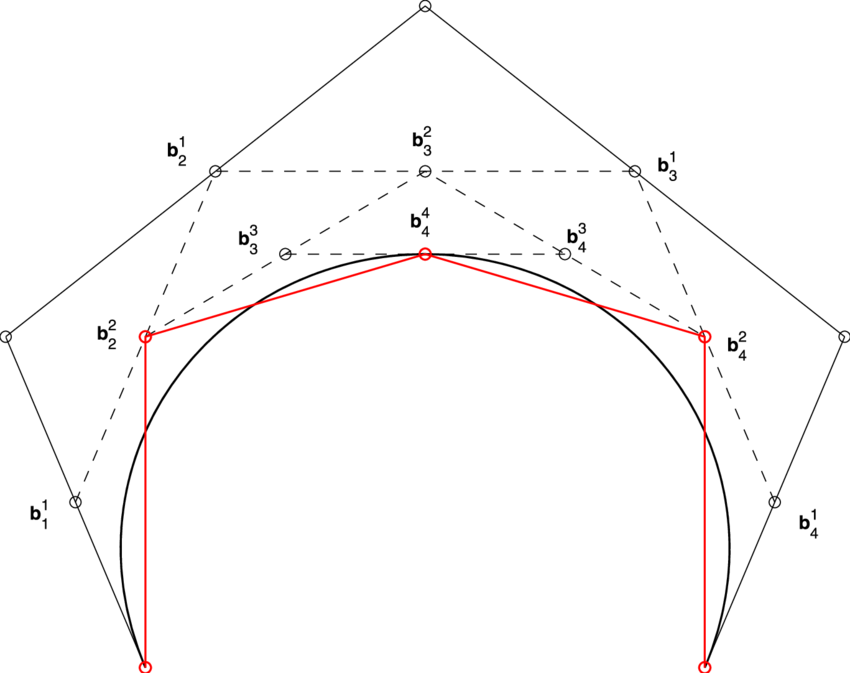
\includegraphics[scale=1]{img/1.png}
	\end{center}
	\caption{}\label{fig:}
\end{figure}

subsubsection{de Rham Curce Continuity}

\begin{property}[Continuity]
	when $0<\lambda _{i,k},\mu_{i,k},\lambda_{i,k}+\mu_{i,k}<1$,de Rham curves $S_k$ is continuted。Assum that $<p_{i-1}^{k}p_{i}^{k},p_{i}^{k}p_{i=1}^{k}>$
\end{property}

\begin{property}[Fractional dimension]
	\begin{enumerate}
		\item F has unnumberable many structure
		\item F is not formular, but it's can be described by computer
		\item Different F has the same as topological dimension
		\item F's fractional dimension is larger than it's topological dimension
	\end{enumerate}
\end{property}



\end{document}
